%!TEX root = skripsi.tex
%-----------------------------------------------------------------------------%
\chapter{\babTiga}\label{bab:tiga}
%-----------------------------------------------------------------------------%
%-----------------------------------------------------------------------------%
% Ide, model matematik, rumus, fitur, jangan m=ngomongin teknologi (java, keras, dll), word2vec boleh %
Pada bab ini \saya~akan menjelaskan metodologi penelitian yang \saya~gunakan. Metodologi penelitian yang dilakukan meliputi tahap pengumpulan data, pra-pemrosesan data, pelabelan data, pengembangan model, eksperimen dan evaluasi.

\section{Gambaran Umum Pengembangan Metodologi}
Penelitian ini bertujuan untuk membuat sebuah model yang mampu memberikan label entitas kesehatan pada suatu dokumen. Seperti yang telah dijelaskan pada bab sebelumnya, terdapat banyak entitas kesehatan yang dapat digunakan sebagai target pelabelan. Oleh karena itu, untuk mempermudah penelitian ini \saya~menggunakan entitas-entitas yang diusulkan oleh \cite{skripsiKakRadit} dalam penelitiannya,  nama penyakit (\textit{\disease}), gejala penyakit (\textit{\symptom}), obat (\textit{\drug}) dan langkah penyembuhan (\textit{\treatment}).

Penelitian ini menggunakan dua buah korpus, yaitu korpus dari data dokumen teks kesehatan yang digunakan \cite{skripsiKakRadit} dan dokumen teks hasil pengumpulan yang dilakukan oleh \saya~pada situs kesehatan \textit{online}. Setelah itu \saya~melakukan pra-pemrosesan pada kedua data sebelum melakukan tahap selanjutnya. Untuk dokumen hasil pengumpulan dari forum, \saya~memberi label kesehatan secara manual dengan ketentuan pelabelan pada penelitian \cite{skripsiKakRadit}

Setelah tahap pengusulan model, terdapat 2 eksperimen \saya~lakukan, yaitu eksperimen untuk mendapatkan fitur diskriminatif yang mampu membuat model memiliki akurasi terbaik dan eksperimen untuk mendapatkan arsitektur RNNs yang membuat model menghasilkan akurasi tertinggi. Pada eksperimen pertama, \saya~mencoba beberapa fitur, seperti fitur yang diusulkan oleh \cite{skripsiKakRadit} (fitur \textit{its own word}, frasa, kamus (\textit{symptom}, \textit{disease}, \textit{treatment} dan \textit{drug}), kata pertama sebelum, dan fitur kata setelah. Pada eksperimen kedua, \saya~mencoba dua arsitektur RNNs, yaitu RNNs yang setiap \textit{input} digabung terlebih dahulu dengan meng-\textit{append} semua vektor fitur. Sedangkan RNNs yang kedua yaitu RNNs yang setiap kelompok fitur menjadi \textit{input} bagi masing-masing LSTMs, baru kemudian \textit{output} dari layer tersebut digabung.

Setelah melakukan eksperimen, \saya~melakukan evaluasi dari hasil yang didapatkan dengan menghitung nilai \textit{precission}, \textit{recall} dan \textit{F-measure} dari masing-masing entitas secara keseluruhan. Untuk mendapatkan rata-rata akurasi dari setiap eksperimen, \saya~melakukan \textit{10-fold cross validation} dengan cara membagi semua data menjadi 10 bagian, 9 bagian menjadi data \textit{training} dan 1 \textit{bagian} menjadi data \textit{testing}. Proses tersebut diulang sebanyak sepuluh kali sehingga masing-masing bagian data menjadi data \textit{testing}.
\begin{figure}
  \centering
  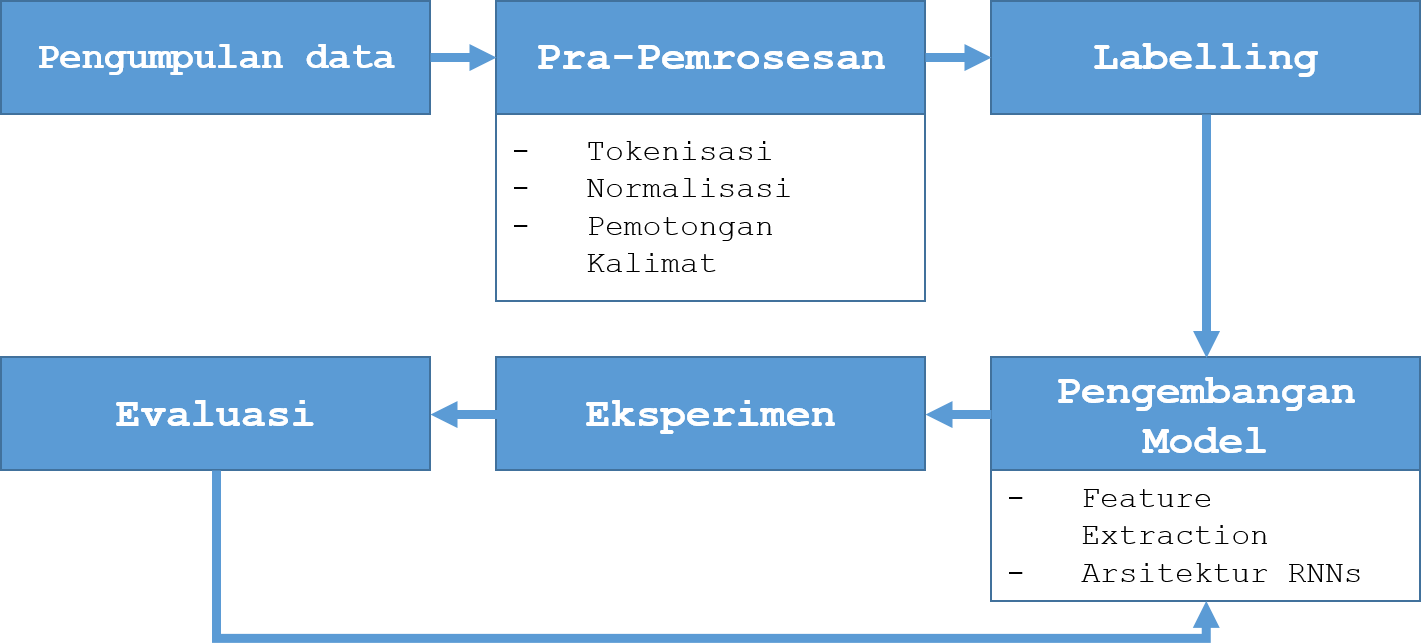
\includegraphics[width=\linewidth]{images/arsitektur}
  \caption{Diagram Gambaran Umum Metodologi yang Dilakukan}
  \label{fig:metodologi_penelitian}
\end{figure}

\section{Pengumpulan Data}
Pengumpulan data dilakukan dengan tujuan untuk mendapatkan data \textit{training} dan \textit{testing} yang akan digunakan sebagai \textit{resource} dalam melakukan \textit{training} dan evaluasi model \mer. Data yang dimaksud merupakan teks dari forum kesehatan \textit{online} dari berbagai sumber. Pada penelitian ini, \saya~menggunakan data penelitian \cite{skripsiKakRadit} dan data yang \saya~dapatkan dari hasil \textit{crawling} di forum kesehatan \textit{online}. Data yang \cite{skripsiKakRadit} diambil dari beberapa situs forim kesehatan \textit{online} dan sedangakn data yang \saya~unduh bersumber dari forum kesehatan \textit{online}.

\section{Pra-Pemrosesan}
Pra-pemrosesan dilakukan dengan tujuan supaya teks yang diberikan mampu dibaca oleh sistem \mer. Dalam tahap ini, ada tiga pekerjaan utama yang perlu dilakukan, yaitu:

\subsection{Pembersihan data}
Langkah ini dilakukan dengan tujuan untuk mempermudah proses POS \textit{tagging}. Selain itu, terdapat beberapa token yang berbeda sintaks namun memiliki jenis kata yang sama, misalnya token \textit{email}. Model hanya perlu tahu token tersebut merupakan email, tidak peduli pemilik email tersebut. Berikut merupakan beberapa langkah yang \saya~lakukan:
	
\begin{enumerate}
	\item menghapus karakter yang bukan merupakan karakter ASCII,
	\item mengganti token url menjadi kata "url", misalnya token tautan (\textit{www.alodokter.com/asma/pengobatan}) diganti menjadi token "url",
	\item mengganti token \textit{email} menjadi kata "email", misalnya sebuah alamat \textit{email} (\textit{wahid@domain.com}) diganti menjadi token "email",
	\item mengganti karakter "\_" menjadi token "underscore",
	\item mengganti karakter "\&" menjadi token "dan",
	\item mengganti karakter "\textless" dan "\textgreater" menjadi token "kurang dari" dan "lebih dari" dan
	\item mengganti karakter "/" menjadi token "atau".
\end{enumerate}
Pada langkah ini, \saya~tidak menghapus karakter tanda baca karena karakter tersebut memiliki fungsi pada sistem POS \textit{tagging} yang \saya~gunakan.
	
\subsection{Tokenisasi}
Tokenisasi dilakukan untuk mendapatkan token yang paling tepat sebagai sebuah kata. Hal ini perlu dilakukan untuk menghindari beberapa kelompok token berbeda yang tergabung. Karakter abjad dengan karakter angka atau karakter abjad dengan karakter tanda baca dipisahkan berdasarkan kelompoknya. Misalnya token "pusing2" diubah menjadi "pusing 2". Pada tahap ini, \saya~melakukan pemisahan terhadap beberapa kelompok token, yaitu:
\begin{enumerate}
	\item <alfabet><numerik> menjadi <alfabet><spasi><numerik>
	\item <numerik><alfabet> menjadi <numerik><spasi><alfabet>
	\item <alfanumerik><non-alfanumerik> menjadi <alfanumerik><spasi><non-alfanumerik>
	\item <alfanumerik><non-alfanumerik> menjadi <alfanumerik><spasi><non-alfanumerik>
\end{enumerate}
	
\subsection{Pemotongan kalimat}
Untuk menghindari jumlah token yang timpang dalam kalimat yang berbeda dan data yang \textit{sparse}, \saya~melakukan pemotongan kata dengan langkah-langkah sebagai berikut:
\begin{enumerate}
	\item memisahkan kalimat berdasarkan tanda baca (.!?,),
	\item apabila suatu kalimat memiliki jumlah kata yang sedikit (batasan minimal jumlah kata dalam sebuah kalimat yang \saya~gunakan adalah 10 kata), kalimat tersebut digabungkan dengan kalimat setelahnya.
\end{enumerate}

\section{Pelabelan}
Pada tahap ini, \saya~melakukan pelabelan pada dokumen teks yang merupakan hasil pada tahap sebelumnya dengan label \disease, \symptom, \drug~dan \treatment. Berikut merupakan penjelasan dari masing-masing label:
\begin{enumerate}
	\item \Disease\\
	Entitas \disease~yang dimaksud pada penelitian ini yaitu nama dari suatu penyakit. Penyakit merupakan keadaan abnormal yang timbul pada tubuh manusia. Contoh dari entitas \disease~yaitu:
	\begin{description}
		\item[$\bullet$] Skizofrenia
		\item[$\bullet$] Trikotilomania
		\item[$\bullet$] Diabetes melitus
	\end{description}

	\item \Symptom\\
	Entitas \symptom~yang dimaksud pada penelitian ini yaitu fenomena yang dialami oleh seseorang yang terkena suatu penyakit. Contoh dari entitas \symptom~yaitu:
	\begin{description}
		\item[$\bullet$] Napas berbunyi
		\item[$\bullet$] Benjolan di daerah perut
		\item[$\bullet$] Nyeri saat BAK
	\end{description}

	\item \Drug\\
	Entitas \drug~merupakan entitas nama obat dari suatu penyakit yang memiliki fungsi untuk mengurangi atau menyembuhkan penyakit tersebut. Contoh dari entitas \drug~yaitu:
	\begin{description}
		\item[$\bullet$] Paracetamol
		\item[$\bullet$] Diltiazem
		\item[$\bullet$] eritropoetin-alfa
	\end{description}

	\item \Treatment\\
	Entitas \treatment~merupakan cara atau langkah penyembuhan dari suatu penyakit. Contoh dari entitas \treatment~yaitu:
	\begin{description}
		\item[$\bullet$] Pemeriksaan darah rutin
		\item[$\bullet$] Penilaian denyut kapiler
		\item[$\bullet$] Terapi inhalasi
	\end{description}
\end{enumerate}
Setelah proses di atas selesai, label di dalam korpus diubah menjadi format BIO (\textit{begin inside outside}).

\section{Pengembangan Model}
Pada tahap ini, \saya~melakukan pengusulan dan perancangan model yang nantinya akan \saya~evaluasi pada tahap eksperimen. Dalam mengembangkan model, terdapat dua pekerjaan yang \saya~lakukan, yaitu:

\subsection{Ekstrasi Fitur}\label{subbab:fitur}
Pada tahap ini, \saya~melakukan ekstraksi fitur dari dokumen yang telah diberi label entitas. Ada beberapa fitur yang \saya~usulkan dalam penelitian ini yang nantinya \saya~kombinasikan supaya mendapatkan hasil terbaik. Fitur-fitur tersebut yaitu:
\begin{enumerate}
	\item Fitur 1: Kata itu sendiri\\
	Fitur ini merupakan fitur kata dalam representasi vektor. Fitur ini merupakan fitur yang digunakan \cite{abacha2011medical} dalam penelitian tentang \mer. Untuk mendapatkan representasi vektor dari masing-masing kata, penulis menggunakan \textit{word embedding}. Pada penelitian mengenai \mer~yang dilakukan oleh \cite{mujiono2016new}, hasil dari representasi data terbaik yaitu \textit{word embedding}. Selain itu, seperti yang dijelaskan pada Bab Tinjauan Pustaka, \textit{word embedding} memberikan hasil yang sangat baik dalam bidang pemrosesan bahasa manusia. Oleh karena itu, \saya~menggunakan \textit{word embedding} untuk mendapatkan representasi vektor masing-masing kata. Dalam penelitian ini. Terdapat beberapa langkah yang perlu \saya~lakukan dalam memanfaatkan \textit{word embedding} ini, yaitu:
	\begin{enumerate}
		\item Pengumpulan data \textit{training} untuk \textit{word embedding}\\
		\Saya~melakukan pengumpulan data teks sebagai \textit{resource} untuk melakukan \textit{training} model \textit{word embedding}. Data teks yang \saya~gunakan merupakan data teks dari artikel-artikel kesehatan dan data teks forum kesehatan di kaskus. \Saya~menggunakan teks berjenis kesehatan supaya \textit{domain word embedding} dengan data \textit{training} untuk model \mer~sama. Selain itu, terdapat beberapa \textit{term} kesehatan yang susah ditemukan di forum umum.
		 
		\item \textit{Training} untuk mendapatkan model \textit{word embedding}\\
		\textit{Training} dilakukan untuk mendapatkan model yang mampu mendapatkan representasi vektor dari sebuah kata. Panjang vektor yang dihasilkan yaitu 1298 dengan besaran \textit{windows} yaitu 5. Arsitektur yang digunakan untuk melakukan \textit{training} ini adalah \textit{skip-gram}.
		
		\item Pengubahan kata menjadi vektor dari model yang didapatkan\\
		Pada langkah ini \saya~mendapatkan suatu kata menjadi representasi vektor dengan model yang telah \saya~dapatkan pada tahap \textit{training} model \textit{word embedding}.
	\end{enumerate}
	
	\item Fitur 2: \textit{Part of Speech Tag} (POS-Tag)\\
	Fitur ini merupakan fitur \textit{tag} yang dimiliki setiap kata yang diusulkan oleh \cite{abacha2011medical} dalam penelitiannya di bidang \mer. Entitas-entitas tertentu memiliki tag yang sama, misalnya entitas obat dan penyakit pada umumnya memiliki tag "NNP" sehingga dengan digunakannya fitur ini sistem dapat mengenali jenis obat dan penyakit dengan lebih baik. Model POS-Tagger yang \saya~gunakan merupakan model POS-Tag berbahasa Indonesia.
	
	\item Fitur 3: \textit{Stopword}\\
	Fitur ini merupakan fitur yang berisi vektor suatu kata merupakan \textit{stopword} atau bukan. Fitur ini \saya~gunakan dalam penelitian ini untuk membantu sistem dalam menghindari kesalahan pelabelan suatu kata yang bukan entitas namun dilabeli sebagai entitas.
	
	Ketika melakukan eksperimen, hasil yang \saya~dapatkan ternyata lebih bagus apabila mempertahankan fitur ini, oleh karena intu, \saya~mengusulkan untuk menggunakan fitur ini. Untuk pembahasan lebih lanjut dibahas pada Bab 5.
	
	\item Fitur 4: Kamus Kesehatan\\
	Fitur kamus kesehatan merupakan fitur yang berisi informasi suatu kata terdapat di dalam kamus kesehatan atau tidak. Pada penelitian ini, kamus kesehatan yang dipakai merupakan kamus \disease, kamus \symptom, kamus \drug~dan kamus \treatment. Dengan menggunakan fitur ini diharapkan mampu berkontribusi dalam meningkatkan akurasi karena model akan mempertimbangkan apakah suatu kata termasuk di dalam kamus atau tidak. 
	
	\item Fitur 5: Frasa Kata\\
	Pada penelitian ini, \saya~mengusulkan fitur frasa kata karena entitas \textit{symptom} dan \textit{treatment}  pada umumnya merupakan frasa kata kerja. Sedangkan entitas \textit{disease} dan \textit{drug} pada umumnya entitas yang akan dikenali pada penelitian ini merupakan frasa kata benda. Oleh karena itu, \saya~berharap bahwa dengan diusulkannya fitur ini akan mampu menambah akurasi dari model yang diusulkan.
	
	Pada penelitian ini ada dua frasa yang diujicobakan, yaitu:
	\begin{enumerate}
		\item Frasa Kata Benda (Nomina)
		Menurut \cite{hs2005bahasa}, frasa kata benda sendiri merupakan kelompok kata benda yang dibentuk dengan memperluas kata benda ke sekelilingnya. Fitur frasa kata benda yang \saya~gunakan dalam penelitian merupakan fitur yang berisi informasi suatu kata atau kumpulan kata merupakan frasa kata benda atau bukan. Dalam menentukan suatu kata merupakan frasa atau bukan, penulis menggunakan aturan pembentukan frasa yang digunakan pada bahasa Indonesia, yaitu:
		\begin{description}
			\item[$\bullet$] NP : NN
			\item[$\bullet$] NP : NNP
			\item[$\bullet$] NP : PR
			\item[$\bullet$] NP : PRP
			\item[$\bullet$] NP : NN + NN
			\item[$\bullet$] NP : NN + NNP
			\item[$\bullet$] NP : NN + PR
			\item[$\bullet$] NP : NN + PRP
			\item[$\bullet$] NP : NN + JJ
			\item[$\bullet$] NP : DT + NN
			\item[$\bullet$] NP : RB + NN
			\item[$\bullet$] NP : CD + NN
			\item[$\bullet$] NP : NND + NN
		\end{description}
		
		\item Frasa Kata Kerja (Verbal)\\
		Menurut \cite{hs2005bahasa}, frasa verbal merupakan kelompok kata benda yang dibentuk dengan kata kerja. Fitur frasa verbal yang \saya~gunakan dalam penelitian merupakan fitur yang berisi informasi suatu kata atau kumpulan kata merupakan frasa verbal atau bukan. Dalam menentukan suatu kata merupakan frasa atau bukan, penulis menggunakan aturan pembentukan frasa yang digunakan pada bahasa Indonesia, yaitu:
		\begin{description}
			\item[$\bullet$] VP : VB
			\item[$\bullet$] VP : VB + NP
		\end{description}
	\end{enumerate}

 \item Fitur 6: 1 Kata Sebelum\\
 Fitur ini merupakan fitur yang berisi informasi kata sebelum kata saat ini yang direpresentasikan dalam bentuk vektor untuk masing-masing kata. Fitur ini digunakan pada penelitian penelitian \cite{skripsiKakRadit} yang juga berkontribusi memberikan hasil terbaik pada penelitiannya. Menurut \saya, ada beberapa entitas yang akan lebih mudah diketahui apabila diketahui kata sebelumnya. Misalnya kata "masuk angin", apabila hanya diberikan informasi kata "angin" tanpa kata "masuk", akan lebih sulit menentukan kata tersebut bagian dari suatu entitas \textit{disease} atau bukan.
  
 \item Fitur 7: 1 Kata Sesudah\\
 Fitur ini merupakan fitur yang berisi informasi kata sesudah kata saat ini yang direpresentasikan dalam bentuk vektor untuk masing-masing kata. Sama seperti pada fitur 1 Kata Sebelum, ada beberapa kasus yang mana apabila suatu kata merupakan sebuah entitas, akan lebih mudah dikenali apabila melihat kata atau konteks setelahnya. Sama seperti contoh pada Fitur 1 Kata Sebelum, misal diberikan kata "masuk angin", apabila hanya diberikan informasi "masuk" tanpa "angin", akan lebih sulit mengenali apakah kata tersebut termasuk entitas \textit{disease} atau bukan. Selain itu, fitur ini juga dapat membedakan kata berentitas dengan kata yang bukan, misalnya kata "masuk angin" dengan "masuk rumah". Apabila informasi pada saat tersebut hanya diberikan kata "masuk" saja tanpa kata setelahnya, akan lebih sulit mengenali kata tersebut termasuk kata berentitas atau bukan.
  
\end{enumerate}

\subsection{Pengusulan Arsitektur RNNs}
Pada tahap ini \saya~mengusulkan arsitektur RNNs yang akan digunakan pada tahap eksperimen. Ada dua arsitektur yang \saya~gunakan dalam penelitian ini, yaitu
\begin{enumerate}
	\item LSTM 1 layer\\
	Pada LSTM 1 layer, semua fitur yang menjadi input pada sebuah \textit{timestep} digabung menjadi satu. Untuk menentukan label, \saya~menggunakan \textit{feed-forward Neural Network} pada masing-masing \textit{timestep} di layer terakhir. Berikut merupakan ilustrasi LSTM 1 layer yang \saya~gunakan dalam penelitian ini.
	
	\begin{figure}
		\centering
		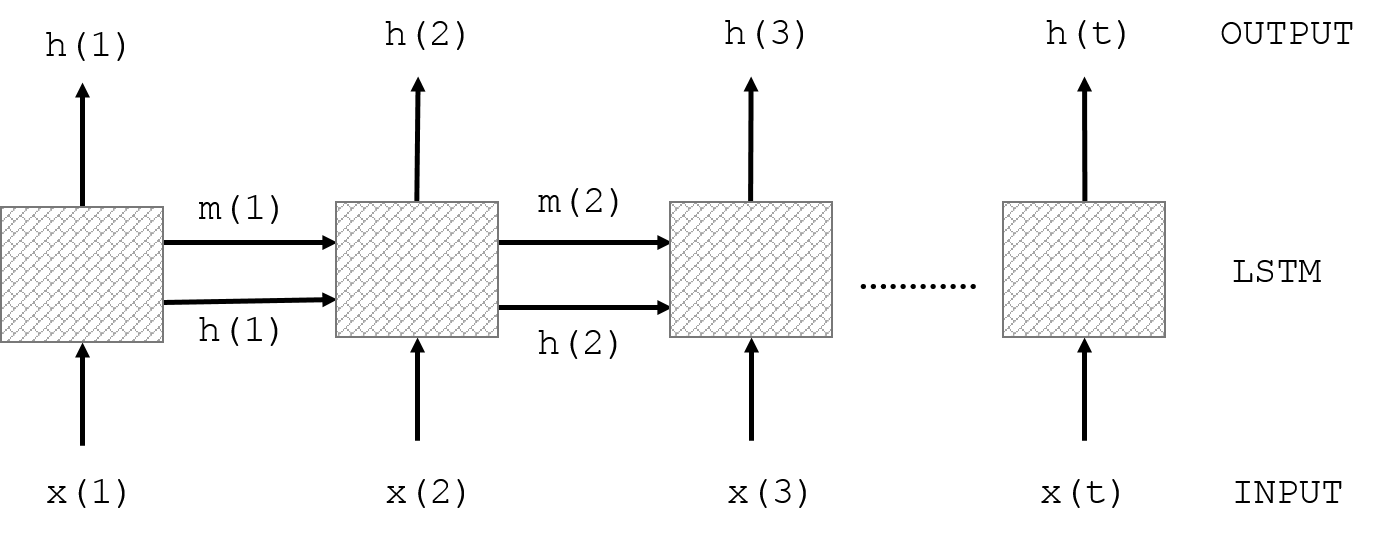
\includegraphics[width=0.8\linewidth]{images/lstm1}
		\caption{LSTM 1 layer}
		\label{fig:single_layer_rnn}
	\end{figure}
	Untuk masing-masing \textit{timestep} $ t $, berikut merupakan gambar sebuah \textit{cell}-nya.
	\begin{figure}
		\centering
		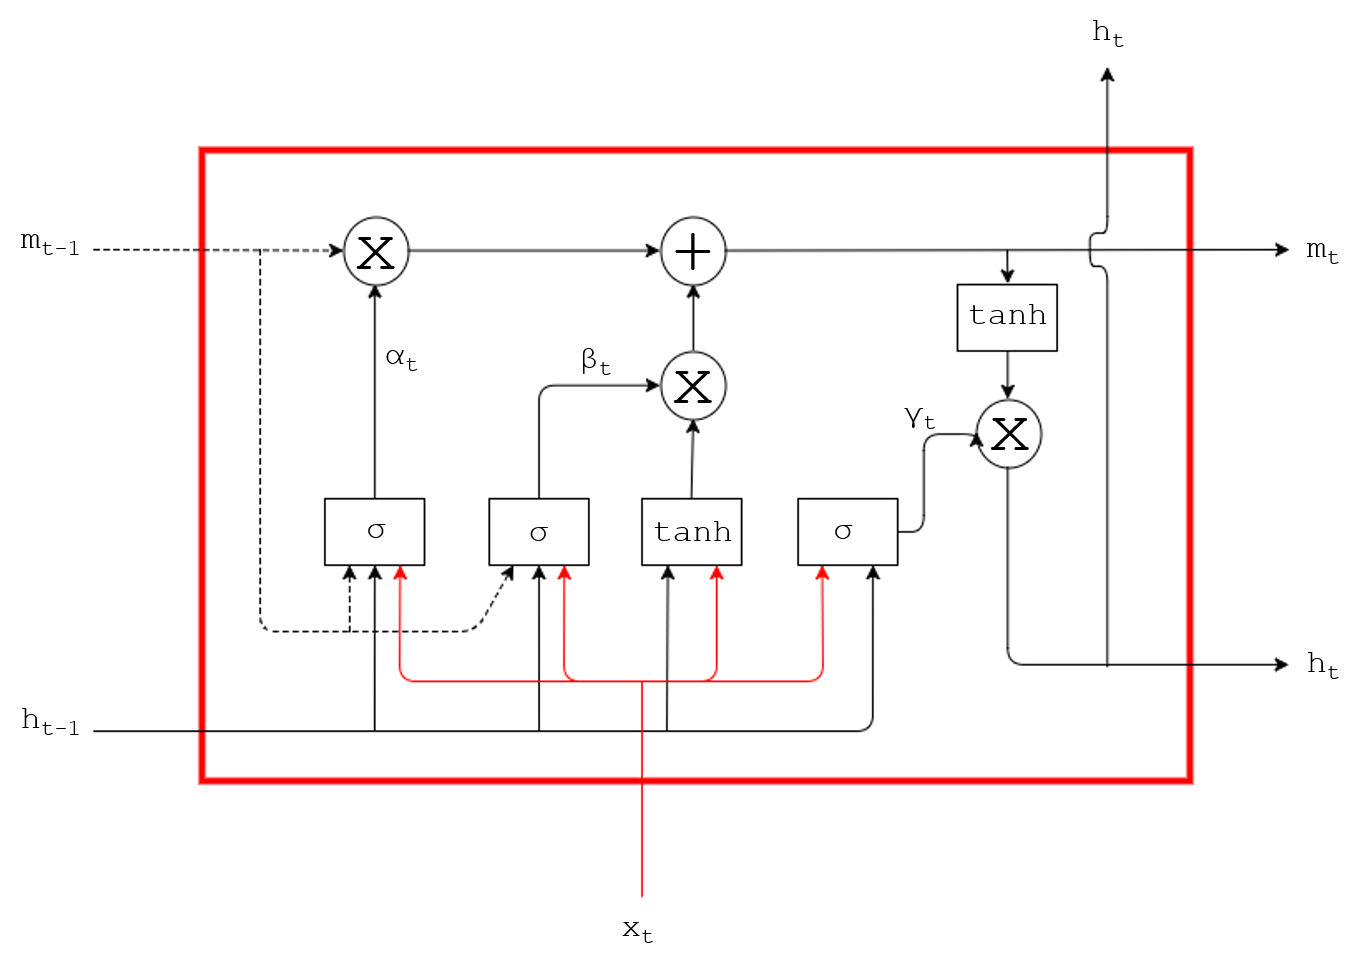
\includegraphics[width=0.85\linewidth]{images/lstm}
		\caption{1 buah blok memori dalam LSTM}
		\label{fig:lstm1cell}
	\end{figure}
	
	Dari gambar \ref{fig:lstm1cell}, sebuah \textit{cell} membutuhkan \textit{input} $ x(t) $ dan \textit{output} $ h(t) $. $ x(t) $ merupakan vektor dengan panjang $ N $, dan $ h(t) $ merupakan vektor dengan panjang $ M $. Seperti yang telah dijelaskan pada subbab \ref{subbab:lstm}, berikut merupakan formula untuk mengetahui \textit{output} pada \textit{timestep} $ t $.
	\begin{equation}\label{eq:lstmm}
	m_{t}=\alpha_{t} (\times) m_{t-1} + \beta_{t} (\times) f(x_{t},{t-1})
	\end{equation}
	\begin{equation}\label{eq:lstmh}
	h_{t}=\gamma_{t} (\times) tanh(m_{t})
	\end{equation}
	dimana
	\begin{equation}\label{eq:lstmx}
	f(x_{t},{t-1})=tanh(W_{xm} \cdot x_{t} + W_{hm} \cdot h_{t-1})
	\end{equation}
	
	$ \alpha_t $, $ \beta_t $ dan $ \gamma_t $ merupakan \textit{gates}:
	\begin{enumerate}
		\item \textit{Forget gates}: $ \alpha_{t}=\tau(W_{x\alpha}+W_{h\alpha}\cdot~h_{t-1}+W_{m\alpha}\cdot~m_{t-1}) $
		\item \textit{Input gates}: $ \beta_{t}=\tau(W_{x\beta}+W_{h\beta}\cdot~h_{t-1}+W_{m\beta}\cdot~m_{t-1}) $
		\item \textit{Output gates}: $ \gamma_{t}=\tau(W_{x\gamma}+W_{h\gamma}\cdot~h_{t-1}+W_{m\gamma}\cdot~m_{t-1}) $
	\end{enumerate}

	\item LSTMs layer bertingkat\\
	Pada LSTMs 2 layer, penulis mendefinisikan 2 tingkat, yang tingkat terbawah merupakan layer dengan jumlah LSTMs sebanyak n kelompok fitur. Pertama-tama fitur dikelompokkan terlebih dahulu, kemudian dijadikan input untuk LSTMs tingkat pertama. Setelah itu, hasil dari tingkat pertama tersebut akan digabung menjadi satu, dengan menggunakan layer penggabung (\textit{Merge Layer}). \textit{Output} dari layer penggabung kemudian dimasukkan ke dalam LSTMa tingkat kedua. Untuk menentukan label, \saya~menggunakan \textit{feed-forward Neural Network} pada masing-masing \textit{timestep} di layer terakhir. Berikut merupakan ilustrasi dari LSTMs layer bertingkat yang \saya~gunakan.
	
	\begin{figure}
		\centering
		\includegraphics[width=1.0\linewidth]{images/lstm2}
		\caption{LSTM 2 layer}
		\label{fig:lstm2}
	\end{figure}

	Masing-masing kelompok fitur menjadi \textit{input} dari LSTMs yang terkait. Nantinya, masing-masing \textit{output} akan digabung melalui \textit{merge layer} dengan metode \textit{concat} dan menjadi \textit{input} bagi LSTMs layer kedua.
	Di sini, \saya~menotasikan $ k $ sebagai nomor kelompok fitur dan $ t $ sebagai \textit{timestep} saat ini. Untuk masing-masing kelompok fitur, berikut merupakan formulasi \textit{feedforward}-nya:
	\begin{equation}\label{eq:mt2}
	m_{k,t}=\alpha_{k,t} (\times) m_{k,t-1} + \beta_{k,t} (\times) f(x_{k,t},{k,t-1})
	\end{equation}
	\begin{equation}\label{eq:ht2}
	h_{k,t}=\gamma_{k,t} (\times) tanh(k,m_{t})
	\end{equation}
	dimana
	\begin{equation}\label{eq:hf2}
	f(x_{k,t},{k,t-1})=tanh(W_{k,xm} \cdot x_{t} + W_{k,hm} \cdot h_{k,t-1})
	\end{equation}
	$ \alpha_{k,t} $, $ \beta_{k,t} $ dan $ \gamma_{k,t} $ merupakan \textit{gates}:
	\begin{enumerate}
	\item \textit{Forget gates}: $ \alpha_{k,t}=\tau(W_{k,x\alpha}+W_{k,h\alpha}\cdot~h_{k,t-1}+W_{k,m\alpha}\cdot~m_{k,t-1}) $
	\item \textit{Input gates}: $ \beta_{k,t}=\tau(W_{k,x\beta}+W_{k,h\beta}\cdot~h_{k,t-1}+W_{k,m\beta}\cdot~m_{k,t-1}) $
	\item \textit{Output gates}: $ \gamma_{k,t}=\tau(W_{k,x\gamma}+W_{k,h\gamma}\cdot~h_{k,t-1}+W_{k,m\gamma}\cdot~m_{k,t-1}) $
	\end{enumerate}

	\textit{Merge layer} berfungsi untuk menggabungkan hasil dari \textit{feedforward} pada semua LSTMs layer pertama. Di sini, saya menotasikan $ X_t $ sebagai hasil dari \textit{merge} di \textit{timestep} $ t $ dan $ (\cdot) $ merupakan operasi \textit{merging}.
	\begin{equation}\label{eq:merge}
	X_t = h_{1,t} (\cdot) h_{2,t} (\cdot) h_{3,t} (\cdot) .... (\cdot) h_{k,t}
	\end{equation}

	Hasil dari \textit{merge layer} akan digunakan sebagai \textit{input} bagi LSTMs tingkat kedua. Untuk memudahkan penggunaan notasi dan membedakan dengan LSTMs pada tingkat pertama, \saya~menggunakan huruf kapital dalam menotasikan masing-masing nilai di LSTMs tingkat kedua. Berikut merupakan formulasi \textit{feed-forwarnya}.
	
	\begin{equation}\label{eq:mt3}
	M_{t}=\alpha_{t} (\times) M_{t-1} + \beta_{t} (\times) f(X_{t},{t-1})
	\end{equation}
	\begin{equation}\label{eq:ht3}
	H_{t}=\gamma_{t} (\times) tanh(M_{t})
	\end{equation}
	dimana
	\begin{equation}\label{eq:hf3}
	f(X_{t},{t-1})=tanh(W_{XM} \cdot X_{t} + W_{HM} \cdot H_{t-1})
	\end{equation}
	$ \alpha_{t} $, $ \beta_{t} $ dan $ \gamma_{t} $ merupakan \textit{gates}:
	\begin{enumerate}
	\item \textit{Forget gates}: $ \alpha_{t}=\tau(W_{X\alpha}+W_{H\alpha}\cdot~H_{t-1}+W_{M\alpha}\cdot~M_{t-1}) $
	\item \textit{Input gates}: $ \beta_{t}=\tau(W_{X\beta}+W_{H\beta}\cdot~H_{t-1}+W_{M\beta}\cdot~M_{t-1}) $
	\item \textit{Output gates}: $ \gamma_{t}=\tau(W_{X\gamma}+W_{H\gamma}\cdot~H_{t-1}+W_{M\gamma}\cdot~M_{t-1}) $
	\end{enumerate}
		
\end{enumerate}
	
\section{Eksperimen}
Dalam melakukan eksperimen, arsitektur \textit{deep learning} yang \saya~gunakan adalah \textit{Recurrent Neural Networks}, dalam hal ini \saya~menggunakan LSTMs. Hal ini \saya~lakukan karena pada penelitian \cite{mujiono2016new}, LSTMs memberikan \textit{output} terbaik dalam \mer~yang dirancang. Selain itu, LSTMs juga sangat baik dalam masalah \textit{sequence labeling} seperti yang dilakukan oleh \cite{graves2013speech} dan merupakan \textit{state-of-the-art} dalam bidang ini. Masih banyak penelitian lain yang membuktikan bahwa LSTMs merupakan arsitektur \textit{deep learning} yang sangat baik dalam masalah \textit{sequence labeling} seperti \textit{Offline Hadwriting Recognition} \citep{graves2009offline}, \textit{sequence tagging} \citep{huang2015bidirectional}, \textit{Sequence to Sequence Learning} \citep{NIPS2014_5346} dan lain lain.

Eksperimen yang \saya~lakukan menggunakan 10-\textit{cross fold validation}, karena keterbatasan data \textit{training} yang \saya~miliki. Sebelum melakukan eksperimen, \saya~membagi data \textit{training} menjadi 10 bagian, kemudian melakukan iterasi sebanyak 10 kali yang pada masing-masing iterasi ke-i, bagian data ke-i menjadi data \textit{testing} dan yang lainnya digabung menjadi data \textit{training}. 

Setelah melakukan pembagian dan pengelompokan data berdasarkan nomor iterasi, penulis membuat model dari data \textit{training} tersebut. Setelah \saya~mendapatkan model, \saya~melakukan testing terhadap masing-masing model dengan data \textit{testing} yang telah disediakan sebelumnya. Hasil dari pelabelan data \textit{testing} ini akan \saya~evaluasi di tahap selanjutnya. Setelah itu \saya~kembali melakukan pembuatan model dengan fitur yang berbeda, atau dengan tambahan fitur lain. Dalam perjalanan melakukan pengujian, apabila fitur yang diuji memberikan hasil yang bagus atau menambah akurasi, \saya~menggabungkan fitur ini ke percobaan selanjutnya. Namun apabila fitur pada saat ini memberikan akurasi yang lebih jelek, \saya~tidak menggunakan fitur tersebut di percobaan selanjutnya.

\subsection{Evaluasi}
Pada tahap ini, \saya~melakukan serangkaian evaluasi dari data \textit{testing} yang telah dilabeli dengan model yang dihasilkan pada tahap eksperimen. \Saya~melakukan evaluasi dengan menggunakan metode \textit{partial evaluation} di mana sebuah token yang diprediksi entitas oleh model dihitung benar apabila terdapat fragmen yang menyusun entitas bernama tersebut \citep{seki2003probabilistic}. Aturan yang \saya~gunakan dalam melakukan evaluasi adalah sebagai berikut: 

\begin{enumerate}
	\item Perhitungan nilai \textit{True Positive} (TP)\\
	Untuk masing-masing kata yang mendapat label entitas benar, nilai $ TP $ bertambah sejumlah kata yang diprediksi benar.\\
	Misal:
	
	\fbox{%
		\parbox{1.0\linewidth}{%
		Contoh 1\\
		True: Bu Ani <Disease>\textbf{sakit kepala} sebelah</Disease>\\
		Predicted: Bu Ani <Disease>\textbf{sakit kepala}</Disease> sebelah
		}%
	}
	
	Dari contoh di atas, nilai $ TP = 2 $, karena ada 2 kata yang mendapatkan label entitas yang benar.
	
	\fbox{%
		\parbox{1.0\linewidth}{%	
		Contoh 2\\
		True : <Disease>Masuk angin</Disease> dan <Sympton>\textbf{suhu badan tinggi}</Symptom>\\
		Predicted : <Sympton>Masuk angin</Sympton> dan <Sympton>\textbf{suhu badan tinggi}</Symptom>\\
		}%
	}

	Dari contoh di atas, nilai $ TP = 3 $, karena ada 3 kata yang mendapatkan label entitas yang benar
	
	\item Perhitungan nilai \textit{False Positive} (FP)\\
	Untuk masing-masing kata yang mendapat label entitas namun seharusnya tidak berentitas,  nilai $ FP $ bertambah sejumlah kata yang diprediksi salah.\\
	Misal:
	
	\fbox{%
		\parbox{1.0\linewidth}{%	
		Contoh 1\\
		True : <Disease>Sakit kepala</Disease> sudah \textbf{beberapa hari istirahat}\\
		Predicted : <Disease>Sakit kepala</Disease> sudah <Treatment>\textbf{beberapa hari istirahat}</Treatment>
		}
	}

	Dari contoh di atas, nilai $ FP = 3 $, karena ada 3 kata yang mendapat label entitas yang seharusnya tidak berlabel, yaitu "beberapa hari istirahat".
			
	\item Perhitungan nilai \textit{False Negative} (FN)\\
	Untuk masing-masing kata yang mendapat label entitas salah,  nilai $ FP $ bertambah sejumlah kata yang diprediksi salah.\\
	Misal:
	
	\fbox{%
		\parbox{1.0\linewidth}{%
		Contoh 1\\
		True : Bu Ani <Disease>sakit kepala sebelah</Disease>\\
		Predicted : Bu Ani <Disease>sakit kepala</Disease> sebelah

		}
	}

	Dari contoh di atas, nilai $ FN = 0 $, karena tidak ada kata yang mendapat label entitas salah (kata "sebelah" tidak mendapat label).
	
	\fbox{%
		\parbox{1.0\linewidth}{%
		Contoh 2\\
		True : <Symptom>Badan terasa pegal</Symptom>, sepertinya akan <Disease>\textbf{demam}</Disease>.\\
		Predicted : <Symptom>Badan terasa pegal</Symptom>, sepertinya akan <Symptom>\textbf{demam}</Symptom>.
		}
	}

	Dari contoh di atas, nilai $ FN = 1 $, karena ada 1 kata yang mendapat label entitas salah, yaitu kata "demam".
	
\end{enumerate}
	
Setelah mendapatkan angka $ TP, FP $ dan $ FN $, \saya~menghitung \textit{f-measure}, \textit{precission} dan \textit{recall} untuk masing-masing entitas dengan menggunakan formula:
\begin{align}
	Precission &= \frac{TP}{TP+FP}\\
	Recall &= \frac{TP}{TP+FN}\\
	F-Measeure &= 2 \cdot \frac{Precission \cdot Recall}{Precission + Recall}
\end{align}

Angka-angka hasil evaluasi ini akan menjadi pertimbangan untuk penggunaan fitur pada saat ini di eksperimen selanjutnya. Apabila akurasi dari penggunaan fitur saat ini lebih baik atau meningkat dari eksperimen sebelumnya, \saya~menggunakan fitur ini pada eksperimen selanjutnya. Selain itu, \saya~juga mengevaluasi arsitektur RNNs yang \saya~gunakan dengan cara yang sama.
	